\chapter{Algorithms}

\subsection{Implementation Steps}
\begin{itemize}
    \item \textbf{Data Preparation: } The dataset was split into X as all the audio features and region and Y as popular.
    The popular column used as the target variable. Then the dataset is split into training and testing sets using an 80-20 split.
    \item \textbf{Feature Scaling: } Features were scaled using the \textit{StandardScaler} from the \textit{sklearn.preprocessing} library to 
    normalize the data and to ensure that all feautres contribute equally to the distance calculation involved in the model, which helps improve the convergence of the algorithm.
    \item \textbf{Handling Class Imbalancae: } To address potential class imbalance in the dataset, the \textit{Synthetic Minority Over-sampling Technique (SMOTE)} was applied, which
    created synthetic samples of the minorty class (popular songs).
    \item \textbf{Model Training: } The algorithm models were trained using the scaled training set. The model was
    configured with a maximum iteration limit of 2000 and class weight balanced to give equal importance to both classes during the training.
    \item \textbf{Cross-Validation: } To evaluate the model's performance more robustly, 5-fold cross-validation was performed.
    This technique involves splitting the data into five subsets (folds) and training the model on four folds while validating it on the remaining
    fold. This process is repeated five times, each time using a different fold for validation.
    \item \textbf{Predictions: } Predictions were made on the scaled test set, and probabilities were calculated for class membership. A threshold of 0.3 was used to adjust the predicted probabilities to determine class labels.
    \item \textbf{Model Evaluation: } The model was evaluated using the confusion matrix, classification report, which included metrics such as precicion, recall, and F1-score.
    \item \textbf{Feature Importance: } The feature importance of the model was determined by examining the coefficients of the models. Both feature importance for whole dataset and feature importance for each specific region has been applied. As a result of this dominant features to determine populartiy of the songs were found.
    \item \textbf{Regional Analysis: } Regional analysis was performed to better understand how different audio features contribute to song populartiy across various regions.
\end{itemize} 


\newpage


\section{Logistic Regression}
Logistic regression is one of the supervised machine learning algorithms to
compute classification problems where the output is binary.
It is based on the idea of modeling the probability of a certain class or event, in this case whether the song will be popular or not with the values of 0 and 1.
Unlike linear regression which predicts continuous values, logistic regression predicts categorical outcomes by applying a logistic function to the input data.
In this project's case, logistic regression is used to predict
whether a song will be popular or not depends on where it will be released and the 
audio features of the song. Logistic regression is a statistical method for 
predicting binary outcomes from the data. The output of the logistic regression is values
either 0 or 1, which 0 represents the song most probably will not be popular and 
1 represents the song most probably will be popular. \\



Accuracy: \textbf{85.42\%}

% Confusion Matrix
% \begin{table}[h]
%     \centering
%     \begin{tabular}{cc|c|c|}
%         \toprule
%         & & \multicolumn{2}{c}{Predicted} \\
%         \cline{3-4}
%         & & 0 & 1 \\
%         \hline
%         \multirow{2}{*}{\textbf{Actual}} & 0 & 55340 & 0 \\
%         & 1 & 9613 & 0 \\
%         \bottomrule
%     \end{tabular}
%     \caption{Confusion Matrix}
%     \label{tab:confusion_matrix}
% \end{table}

Classification Report
\begin{table}[h]
    \centering
    \begin{tabular}{lcccc}
        \toprule
        & \textbf{Precision} & \textbf{Recall} & \textbf{F1-score} & \textbf{Support} \\
        \midrule
        0 & 0.85 & 1.00 & 0.92 & 55340 \\
        1 & 0.00 & 0.00 & 0.00 & 9613 \\
        \midrule
        \textbf{Accuracy} & \multicolumn{4}{c}{0.85} \\
        \textbf{Macro avg} & 0.43 & 0.50 & 0.46 & 64953 \\
        \textbf{Weighted avg} & 0.73 & 0.85 & 0.78 & 64953 \\
        \bottomrule
    \end{tabular}
    \caption{Classification Report}
    \label{tab:classification_report}
\end{table}

\begin{figure}[h] 
    \centering 
    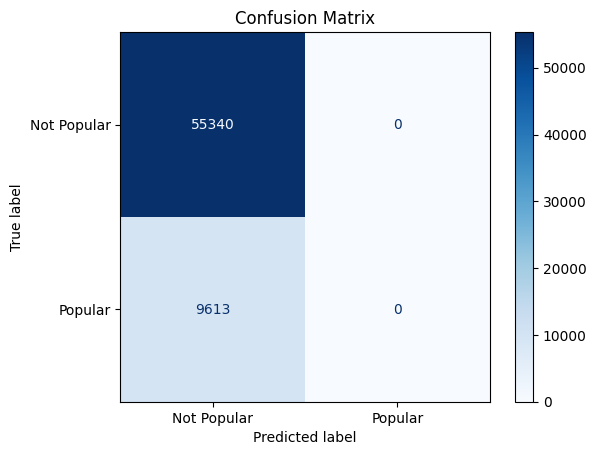
\includegraphics[width=0.6\textwidth]{media/log_reg_confusionmatrix.png}
    \caption{Confusion Matrix of Logistic Regression Model}

\end{figure}



\newpage

\section{Decision Tree}

Decision Tree is a supervised machine learning algorithm that is used for both classification and regression tasks. It works by recursively partitioning the data into subsets based on the values of the input features. The goal is to create a model that predicts the value of the target variable by learning simple decision rules inferred from the data features. Decision trees are easy to interpret and visualize, making them popular for exploratory data analysis and decision-making tasks. In this project, Decision Tree was used to predict whether a song will be popular or not based on their audio features and region affiliation. \\

After splitting the dataset into test and train sets and fitting the model, the Decision Tree model was evaluated using the following metrics: accuracy, confusion matrix and classification report.


Accuracy: \textbf{75.97\%}

Classification Report
\begin{table}[h]
    \centering
    \begin{tabular}{lcccc}
        \toprule
        & \textbf{Precision} & \textbf{Recall} & \textbf{F1-score} & \textbf{Support} \\
        \midrule
        0 & 0.87 & 0.85 & 0.86 & 55340 \\
        1 & 0.22 & 0.25 & 0.23 & 9613 \\
        \midrule
        \textbf{Accuracy} & \multicolumn{4}{c}{0.76} \\
        \textbf{Macro avg} & 0.54 & 0.55 & 0.55 & 64953 \\
        \textbf{Weighted avg} & 0.77 & 0.76 & 0.77 & 64953 \\
        \bottomrule
    \end{tabular}
    \caption{Classification Report}
    \label{tab:classification_report}
\end{table}
 
\begin{figure}[h] 
    \centering 
    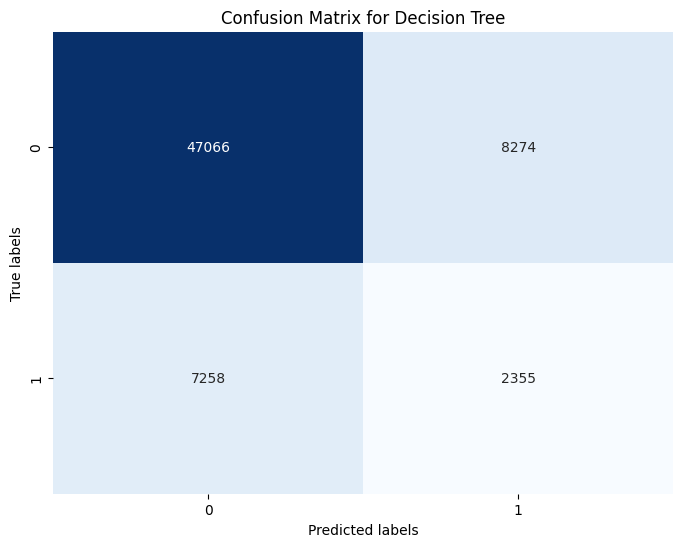
\includegraphics[width=0.6\textwidth]{media/decision_tree_conf_matr.png}
    \caption{Confusion Matrix of Decision Tree Model}

\end{figure}

The Decision Tree Classifier can be shown:

\begin{figure}[H] 
    \centering 
    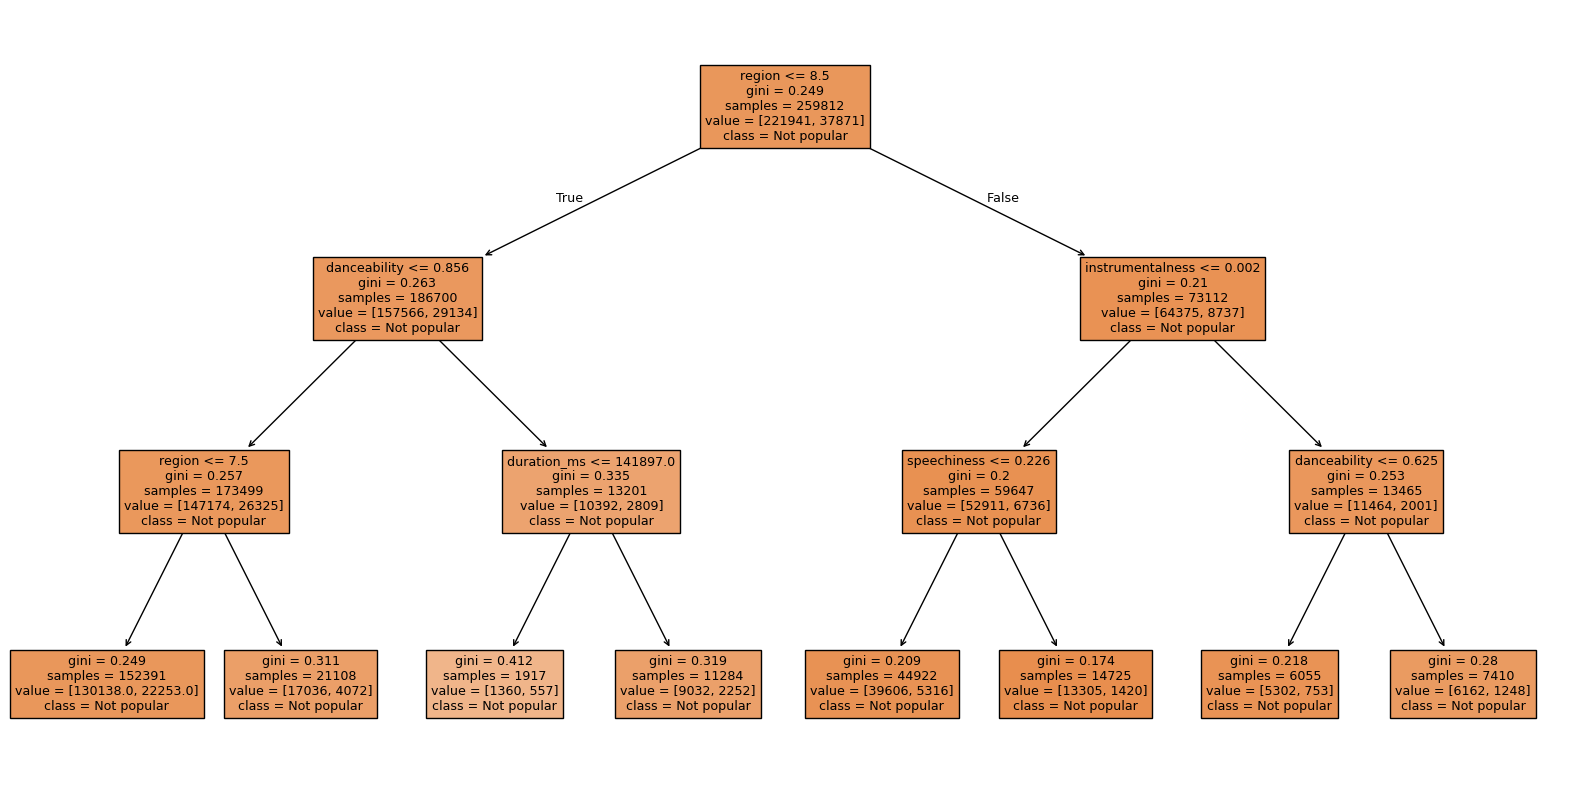
\includegraphics[width=0.9\textwidth]{media/decision_tree.png}
    \caption{Decision Tree Classifier}
    \label{fig:decision_tree}
\end{figure}



\section{Random Forest}
Random Forest is an ensemble learning method that constructs a multitude of decision trees during
training and outputs the mode of the classes as the prediction of the individual trees. Random Forest
is a versatile machine learning algorithm that can be used for both classification and regression
tasks. It is based on the concept of bagging, which involves training multiple models on different
subsets of the data and combining their predictions to improve the overall performance. Random Forest
is known for its robustness, scalability, and ability to handle high-dimensional data with ease.
In this project, Random Forest was used to predict whether the song will be popular or not based on their audio
features and release region. \\
The concept of Random Forest is based on Bagging (Bootsrap Aggregating) which is a technique to reduce the variance of the model
by averaging the predictions of multiple models. Random Forest builds multiple decision trees and merges them together to get a more
accurate and stable prediction.
\\
\\
Mathematically, if \( T_1, T_2, \dots, T_B \) are the \( B \) decision trees in the forest, and \( h(x) \) is the output prediction of a single tree for input \( x \), the Random Forest prediction for classification is:

\[
\hat{y} = \text{mode} \left( T_1(x), T_2(x), \dots, T_B(x) \right)
\]

For regression, the final prediction is the average:

\[
\hat{y} = \frac{1}{B} \sum_{i=1}^{B} T_i(x)
\]
\\
\\
\\
Accuracy: \textbf{85.67\%}

\newpage
Classification Report
\begin{table}[h]
    \centering
    \begin{tabular}{lcccc}
        \toprule
        & \textbf{Precision} & \textbf{Recall} & \textbf{F1-score} & \textbf{Support} \\
        \midrule
        0 & 0.88 & 0.96 & 0.92 & 55340 \\
        1 & 0.53 & 0.26 & 0.35 & 9613 \\
        \midrule
        \textbf{Accuracy} & \multicolumn{4}{c}{0.86} \\
        \textbf{Macro avg} & 0.71 & 0.61 & 0.64 & 64953 \\
        \textbf{Weighted avg} & 0.83 & 0.86 & 0.84 & 64953 \\
        \bottomrule
    \end{tabular}
    \caption{Classification Report}
    \label{tab:classification_report}
\end{table}

\begin{figure}[h] 
    \centering 
    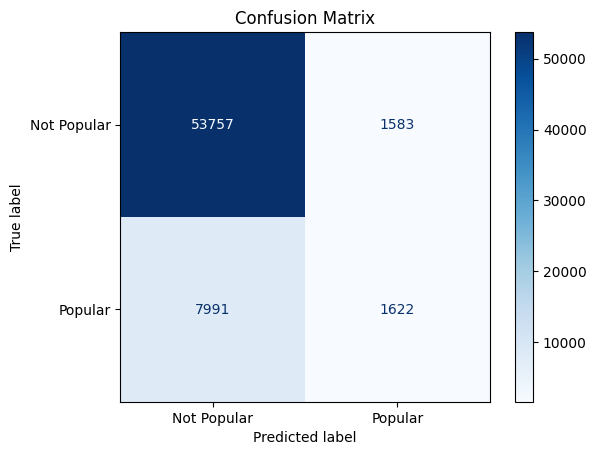
\includegraphics[width=0.6\textwidth]{media/random_forest_conf_matrix.png}
    \caption{Confusion Matrix of Random Forest Model}

\end{figure}




\section{Naive Bayes}
Naive Bayes is a family of probabilistic algorithms based on Bayes' Theorem, which is used for classification tasks.
The algorithm is particularly popular for its simplicity, efficiency, and effectiveness in dealing with large datasets.
It is called "naive" because it makes the assumption that the features are independent of each other given the class label.
In this project Gaussian Naive Bayes is used to predict whether a song will be popular or not based on its audio features and release region by assuming that
the features follow a normal distribution. The fundamental principle of the Naive Bayes algorithm is Bayes' Theorem, which is expressed as:

\[
P(C | X) = \frac{P(X | C) \cdot P(C)}{P(X)}
\]

Where:
\begin{itemize}
    \item \( P(C | X) \) is the posterior probability of class \( C \) given the features \( X \).
    \item \( P(X | C) \) is the likelihood of observing the features \( X \) given class \( C \).
    \item \( P(C) \) is the prior probability of class \( C \).
    \item \( P(X) \) is the prior probability of observing the features \( X \).
\end{itemize}

To make predictions, Naive Bayes calculates the posterior probability for each class and selects the class with the highest probability. The independence assumption simplifies the calculation of the likelihood:

\[
P(X | C) = P(X_1 | C) \cdot P(X_2 | C) \cdots P(X_n | C)
\]

Where \( X_1, X_2, \ldots, X_n \) are the features.

Accuracy: \textbf{85.04\%}


Classification Report
\begin{table}[h]
    \centering
    \begin{tabular}{lcccc}
        \toprule
        & \textbf{Precision} & \textbf{Recall} & \textbf{F1-score} & \textbf{Support} \\
        \midrule
        0 & 0.85 & 1.00 & 0.92 & 55340 \\
        1 & 0.17 & 0.00 & 0.01 & 9613 \\
        \midrule
        \textbf{Accuracy} & \multicolumn{4}{c}{0.85} \\
        \textbf{Macro avg} & 0.51 & 0.50 & 0.46 & 64953 \\
        \textbf{Weighted avg} & 0.75 & 0.85 & 0.78 & 64953 \\
        \bottomrule
    \end{tabular}
    \caption{Classification Report}
    \label{tab:classification_report}
\end{table}

\begin{figure}[h] 
    \centering 
    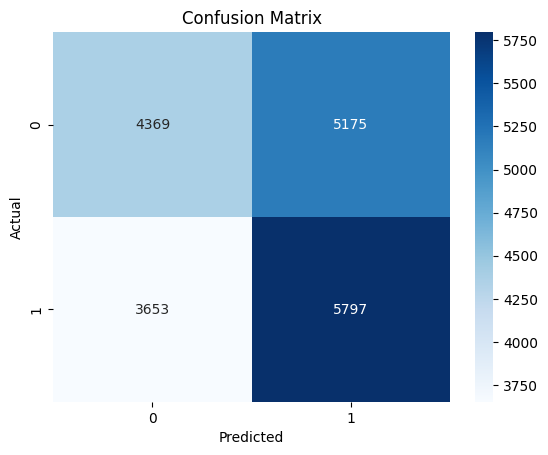
\includegraphics[width=0.6\textwidth]{media/naive_bayes_confusion_matrix.png}
    \caption{Confusion Matrix of Naive Bayes Model}

\end{figure}


\newpage


\section{K-Nearest Neighbors}

Accuracy: \textbf{83.92\%}


Classification Report
\begin{table}[h]
    \centering
    \begin{tabular}{lcccc}
        \toprule
        & \textbf{Precision} & \textbf{Recall} & \textbf{F1-score} & \textbf{Support} \\
        \midrule
        0 & 0.87 & 0.96 & 0.91 & 55340 \\
        1 & 0.39 & 0.16 & 0.22 & 9613 \\
        \midrule
        \textbf{Accuracy} & \multicolumn{4}{c}{0.85} \\
        \textbf{Macro avg} & 0.63 & 0.56 & 0.57 & 64953 \\
        \textbf{Weighted avg} & 0.80 & 0.84 & 0.81 & 64953 \\
        \bottomrule
    \end{tabular}
    \caption{Classification Report}
    \label{tab:classification_report}
\end{table}

\begin{figure}[h] 
    \centering 
    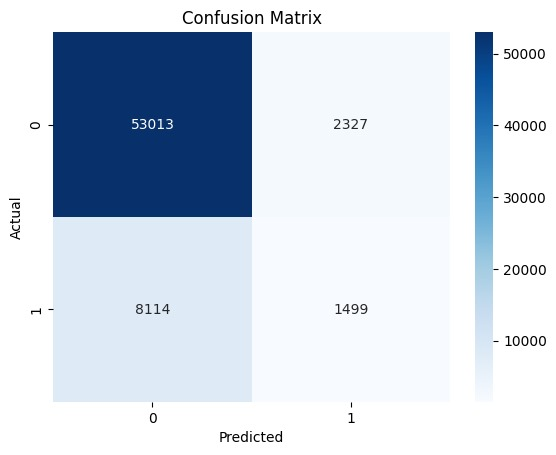
\includegraphics[width=0.6\textwidth]{media/knn-confusion_matrix.jpg}
    \caption{Confusion Matrix of KNN Model}

\end{figure}